\chapter{Homotopy type theory}
\label{chap:hott}

\epigraph{Mathematics is the art of giving the same name to different
  objects.}{Henri Poincaré}

This chapter is an overview of the setting we will use in the rest of
the thesis, homotopy type theory. The first part describes the formal
system {\em dependent type theory}, which is a formal basis for
homotopy type theory. This description is not intended to form a
complete introduction to type theory accessible by anyone, but rather
to clarify the formal system we use. A neophyte willing to read this
thesis should read first a complete introduction to type theory,
\cite{hofmann1997syntax} for an extensive one, but \cite{hottbook}
might be more accessible, and sufficient for the thesis. As we will
see, we can view homotopy type theory as in
\[ 
  \text{HoTT} = \text{MLTT} + \text{UA} + \text{HIT}.
\]
{UA} stands for {\em univalence axiom}, and is introduced in the
second part of this chapter.
{HIT} is the usual abbreviation for {\em higher inductive types},
which is a way, extensively discussed in~\cite{hottbook}, to build new
type, by giving constructors for the type as well as for its identity
types. General principles will not be discussed here ; we
rather present usual examples of {HIT} in section~\ref{sec:hit}.

Finally, the last section of this chapter presents our point of view
on identity paths, leading to the terminology {\em homotopy} type
theory. This section also introduces the notion of {\em truncation
  level}, which plays a central role in the thesis. 


\section{Dependent type theory}
\label{sec:mltt}

In Zermelo-Frank\ae l set theory, the most basic assertion is
\[ x\in E\]
where $x$ and $E$ are sets. 
In dependent type theory, a similar judgement can be
\[a:A, \]\nomenclature{$a:A$}{Judgement ``$a$ is of type $A$''}
to be read as ``$a$ is of type $A$''. The main difference with
membership relation is that an element $a$ has one and only one type,
while we can say $x\in E$ and $x\in F$ for the same element $x$ in set
theory (it is the definition of $x\in E\cap F$).

Dependent (or Martin-L\'of, due to its inventor~\cite{mltt}) type
theory is based on the Curry-Howard correspondance~\cite{Howard80}, or
propositions-as-types principle. Indeed, we do not need to make a
difference between types an propositions. Hence $a:A$ will be read
``$a$ is of type $A$'' when $A$ is seen as a type, and ``$a$ is a
proof of $A$'' when $A$ is seen as a proposition. In the rest of this
section~\ref{sec:mltt}, we present the different types used to build
dependent type theory. It is not intended to be complete ; for example
we sometimes only give the non-dependent elimination rules to ease the
reading. The reader
can refer to~\cite{nordstrom2001martin} or~\cite{hottbook} for a more
detailed introduction.


\subsection{Universes}
\label{ssec:universes}
In dependent type theory, types are also terms of a universe
$\Type$. Of course, we want the universe $\Type$ to be itself a type,
and the Russel's paradox\footnote{In type theory, the argument is
  harder to prove, and is called Girard's paradox.} is close here.
We solve the problem by using a cumulative hierarchy of universes
\[ \Type^0 : \Type^1 : \Type^2 :\cdots \]
\nomenclature{$\Type^i$}{$i$-th universe}
where every universe $\Type^i$ is of type $\Type^{i+1}$. Cumulativity means
that if $A:\Type^k$ and $k<m$, then $A:\Type^m$. The handling of
universes level can be done automatically\footnote{We will see in
  chapters~\ref{chap:modalities} and~\ref{chap:sheaf} that we
  sometimes need to ``help'' Coq}
 by proof assistants such as Coq,
and we will thus use only a ``type of type'' $\Type$, to be understood
in a polymorphic way.

\subsection{Empty and Unit types}
\label{ssec:unit_empty}

The first two types we will see are the Empty type (denoted
$\zero$\nomenclature{$\zero$}{Empty type}) and the Unit type (denoted
$\one$\nomenclature{$\one$}{Unit type}).
These are respectively the types with zero and one elements (named $\unittt$). Those two
types are dual to each other:
\begin{itemize}
\item having a term of type $\zero$ in the context allows to prove
  anything, while having a term of type $\one$ in the context is
  useless
\item dually, giving a term of type $\one$ is trivial, while giving a
  term of type $\zero$ is impossible (if the theory if consistent).
\end{itemize}

Here are the (non-trivial) introduction and elimition rules for these types:

\begin{center}
  \AxiomC{$\Gamma\vdash x:\zero$}
  \AxiomC{$X:\Type$}
  \RightLabel{$\zero$-\textsc{elim}}
  \BinaryInfC{$\Gamma \vdash X$}
  \DisplayProof
  \qquad
  \AxiomC{}
  \RightLabel{$\one$-\textsc{intro}}
  \UnaryInfC{$\Gamma\vdash \unittt:\one$}
  \DisplayProof
\end{center}

Under the propositions-as-types principle, $\zero$ is the type always
false, and $\one$ the type always true. With a categorical point of
view, $\zero$ is an initial object and $\one$ is a terminal object.

\subsection{Coproduct}
\label{ssec:coproduct}

The coproduct of $A$ and $B$, noted $A+B$\nomenclature{$A+B$}{Coproduct of
  types}, is seen as the disjoint sum of $A$ and $B$. It is described
by the inductive type generated by
\[ \left|
    \begin{array}{lll}
      \inl & : & A \to A+B \\
      \inr & : & B \to A+B
    \end{array}
  \right. \]

The introduction and elimination rules of coproduct are:
\begin{center}
  \AxiomC{$\Gamma\vdash a:A$}
  \RightLabel{$+$-$\textsc{intro}_L$}
  \UnaryInfC{$\Gamma\vdash \inl a : A+B$}
  \DisplayProof
  \qquad
  \AxiomC{$\Gamma\vdash b:B$}
  \RightLabel{$+$-$\textsc{intro}_R$}
  \UnaryInfC{$\Gamma\vdash \inr b : A+B$}
  \DisplayProof
  \vspace{1em}

  \AxiomC{$\Gamma\vdash p:A+B$}
  \AxiomC{$\Gamma,x:A\vdash c_A:C$}
  \AxiomC{$\Gamma,x:B\vdash c_B:C$}
  \RightLabel{$+$-\textsc{elim}}
  \TrinaryInfC{$\Gamma,\vdash\mathrm{sum\_rect}(p,c_A,c_B) : C$}
  \DisplayProof
\end{center}

Under the propositions-as-types principle, $A+B$ is seen as the
disjunction of $A$ and $B$.

\subsection{Dependent product}
\label{ssec:pi}
One of the things both mathematicians and computer scientists love to
do is to define functions. If $A$ and $B$ are types, one can consider
the type of functions from $A$ to $B$, taking an inhabitant of type
$A$ (called the source type) and giving an inhabitant of type $B$ (the
target type). What is new in dependent type theory
is that the target type is allowed to depend on the argument of the
function. 

\begin{exm}
  For example, one can consider a function taking a natural number $n$
  and giving a natural number greater than $n$. The target source
  depends indeed of $n$.
\end{exm}

The type of dependent functions with source type $A$ and target type
$B\, x$ is called ``dependent product over $B$'' (or ``pi-type over
$B$''), and will be denoted $\prodD x A {B\, x}$\nomenclature{$\prodD a A
  {B\, a}$}{Dependent product over $B$} or $(x:A)\to (B\,
a)$\nomenclature{$(x:A)\to (B\, a)$}{Dependent product over $B$}.
When $B$ does not depend on $A$, we just say ``arrow type'' and note
it $A\to B$\nomenclature{$A\to B$}{Type of arrows from $A$ to $B$}.

The introduction and elimination rules of dependent products are:

\begin{center}
  \AxiomC{$\Gamma,x:A\vdash b:B$}
  \RightLabel{$\prod$-\textsc{intro}}
  \UnaryInfC{$\Gamma\vdash \lambda\, (x:A),\, b : \prodD x A B$}
  \DisplayProof
  \qquad
  \AxiomC{$\Gamma\vdash f:\prodD x A B$}
  \AxiomC{$\Gamma\vdash a:A$}
  \RightLabel{$\prod$-\textsc{elim}}
  \BinaryInfC{$\Gamma\vdash f(a):B[a/x]$}
  \DisplayProof
\end{center}

Under the propositions-as-types, type of non-dependent functions $A\to
B$ is seen as implication $A\To B$, and type of dependent functions
$\prodD x A {B\, x}$ is seen as universally quantified formulas
$\forall x,\, B\, x$.

\subsection{Dependent sum}
\label{ssec:sigma}

If $A$ and $B$ are two types, we would like to define the type of
pairs $(a,b)$, where $a:A$ and $b:B$. The resulting type is called the
product of $A$ and $B$, noted $A\times B$\nomenclature{$A\times
  B$}{Product of types}.

As for functions, dependent type theory allows the second type to
depend on the first type. Thus, the type of pairs where the first
element $x$ is in type $A$ and the second element $y$ is in type $B\,
x$ is called ``dependent sum over $B$'' (or sigma-type over $B$), noted $\sumD
a A {B\, a}$\nomenclature{$\sumD a A {B\, a}$}{Dependent sum over
  $B$}.

The introduction and elimination rules are:

\begin{center}
  \AxiomC{$\Gamma,x:A\vdash B:\Type$}
  \AxiomC{$\Gamma\vdash x:A$}
  \AxiomC{$\Gamma\vdash b:B[a/x]$}
  \RightLabel{$\sum$-\textsc{intro}}
  \TrinaryInfC{$\Gamma\vdash (a,b):\sumD x a B$}
  \DisplayProof
  \vspace{1em}

  \AxiomC{$\Gamma\vdash p:\sumD x A B$}
  \RightLabel{$\sum$-$\textsc{intro}_1$}
  \UnaryInfC{$\Gamma\vdash \pi_1 p: A$}
  \DisplayProof
  \qquad
  \AxiomC{$\Gamma\vdash p:\sumD x A B$}
  \RightLabel{$\sum$-$\textsc{intro}_2$}
  \UnaryInfC{$\Gamma\vdash \pi_2 p: B[\pi_1 p/x]$}
  \DisplayProof
\end{center}

The projections $\pi_1$ and $\pi_2$ will sometimes be noted, when
applied to a term $u$, $u_1$ and $u_2$.

\begin{rmq}
  We note that the terminology might be confusing: the dependent
  generalization of products are dependent sums, while dependent
  products are generalization of functions.
\end{rmq}

Under the propositions-as-types principle, $A\times B$ is seen as the
conjonction $A\land B$, and $\sumD x A {B\, a}$ is seen as the
existentially quantified formula $\exists x\, B\, x$.

If $A$ and $B$ are types, $f:A\to B$ and $b:B$, the particular
dependent sum $\sumD a A {f\, a = b}$ is called the fiber of $f$ over
$b$, noted $\fib f b$\nomenclature{$\fib f b$}{Fiber of $f$ over
  $b$}. It describes the inverse image of $b$ by $f$.

\subsection{Inductive types}
\label{ssec:inductive}

Dependent type theory actually allows us to define any inductive
type. An inductive type is a type defined only by its introduction
rules, in a free way. Its elimination rules are automatically
determined. We have already seen examples of inductive types: Empty,
Unit, Coproduct.

The most basic example of inductive types might be the type
$\N$\nomenclature{$\N$}{Type of naturals} of naturals. Its
introduction rules are

\begin{center}
  \AxiomC{}
  \RightLabel{$\N$-$\textsc{intro}_0$}
  \UnaryInfC{$0:\N$}
  \DisplayProof
  \qquad
  \AxiomC{$\Gamma\vdash n:\N$}
  \RightLabel{$\N$-$\textsc{intro}_S$}
  \UnaryInfC{$\Gamma \vdash S\, n : \N$}
  \DisplayProof
\end{center}

We also say that its {\em constructors} are $0:\N$ and $S:\N\to
\N$: $\N$ is thus the free monoid generated by $0$ and $S$.
The elimination rule for $\N$ is the famous induction principle

\begin{center}
  \AxiomC{$\Gamma,x:\N\vdash P:\Type$}
  \noLine
  \UnaryInfC{$\Gamma\vdash n:\N$}
  \AxiomC{$\Gamma\vdash c_0:C[0/x]$}
  \noLine
  \UnaryInfC{$\Gamma,n:\N,y:C \vdash c_S : C[S\, n/x]$}
  \RightLabel{$\N$-\textsc{elim}}
  \BinaryInfC{$\Gamma\vdash \mathrm{nat\_ind}(C,c_0,c_S(n,y),n) : C[n/x]$}
  \DisplayProof
\end{center}

This elimination rule allows us to define basic operators on natural
numbers: addition, multiplication, order, \etc{}

For a reader interested by the theory of general inductive types, we
refer him to~\cite{awodey-inductive}.

\subsection{Paths type}
\label{ssec:path}
One of the most powerful tool in dependent type theory might be the
identity types. They allow us to talk about propositional equality
between inhabitants of a type. The identity type over $A$ will be
noted $a=_A b$ or $a=b$ if $A$ can be inferred from context
\nomenclature{$a=_A b$}{Type of paths from $a$ to $b$ in
  $A$}\nomenclature{$a=b$}{Type of paths from $a$ to $b$}. What is
great about identity type over $A$ is that its definition does not
depend on the type $A$. If $a,b:A$, $a=_A b$ is defined as the
inductive type whose only constructor is \[\idpath:\prodD a A {a=_A a}\]
($\idpath_x$ will sometimes be just noted $1_x$, or even
$1$)\nomenclature{$\idpath_x$ or $1_x$}{Constant path
  over$x$}\nomenclature{$\idpath$ or $1$}{Constant path}.

\begin{center}
  \AxiomC{$\Gamma\vdash a:A$}
  \RightLabel{$=$-\textsc{intro}}
  \UnaryInfC{$\Gamma\vdash \idpath_a : a =_A a$}
  \DisplayProof
  \vspace{1em}

  
  \AxiomC{$\Gamma\vdash a,b:A$}
  \noLine
  \UnaryInfC{$\Gamma\vdash q:a=_A b$}
  \AxiomC{$\Gamma,x:A,y:A,p:x=_A y\vdash P:\Type$}
  \noLine
  \UnaryInfC{$\Gamma,z:A\vdash w:P[z,z,1/x,y,p]$}
  \RightLabel{$=$-\textsc{elim}}
  \BinaryInfC{$\Gamma\vdash \mathrm{path\_ind}_P^q(w) : P[a,b,q/x,y,p]$}
  \DisplayProof
\end{center}

The elimination principle should be looked closer. Lets simplify to
understand how it works: suppose that the type family $P$ depends only
on two objects $x,y:A$. Then if $C$ is reflexive, \ie{} if $C(x,x)$ is
always inhabited, then whenever $x=y$, $C(x,y)$ is inhabited too.

Path-induction, also known as ``$J$ principle'', allow us to state
the following:
\begin{lem}[{\cite[Lemma 2.3.1]{hottbook}}]
  Let $A:\Type$ and $P:A\to\Type$ a type family over $A$. Then if
  $p:x=_A y$, there is a function $\transport_P^p :P\, x\to P\, y$.
\end{lem}
\begin{proof}
  Let's do this proof to use path-induction for the first time. Let
  $Q$ be the type family indexed by $x,y:A$ 
  \[ Q(x,y) := P\, x \to P\, y. \]
  Then by path-induction, it suffices to define $Q(x,x)$. The latter
  is clearly inhabited by $\idmap_{P\, x}$.
\end{proof}

Path-induction might be the most powerful tool we can use. For
example, most of the lemmas we will see in section~\ref{sec:hott} can
be proved using path-induction.

\subsection{Summary}
\label{ssec:mltt_summary}

We can summarize the situation in the following array:

\renewcommand{\arraystretch}{2}
\begin{tabular}{|l|l|l|}
  \hline
  Name & Notation & Proposition-as-types \\
  \hline\hline
  Empty & $\displaystyle{\zero}$ & $\displaystyle{\bot}$ \\
  \hline
  Unit & $\displaystyle{\one}$ & $\displaystyle{\top}$ \\
  \hline
  Coproduct, sum & $\displaystyle{A+B}$ & $\displaystyle{A\lor B}$ \\
  \hline
  Function & $\displaystyle{A\times B}$ & $\displaystyle{A\To B}$ \\
  \hline
  Dependent function, pi-type & $\displaystyle{\prodD x A {B\, x}}$ & $\displaystyle{\forall x,\,
                                                       B\, x}$ \\
  \hline
  Product & $\displaystyle{A\times B}$ & $\displaystyle{A\land B}$ \\
  \hline
  Dependent sum, sigma-type & $\displaystyle{\sumD x A {B\, x}}$ & $\displaystyle{\exists x,\, B\,
                                                    x}$ \\
  \hline
\end{tabular}
\renewcommand{\arraystretch}{1}

\section{Identity types and Univalence axiom}
\label{sec:ua}

Identity types are very useful to assert propositional equalities
between object. Note that it does not characterize {\em judgemental}
equality, which we consider here as belonging to the meta-theory (some
theories, as Voevodsky's Homotopy Type System~\cite{hts}, implemented
in proof assistant Andromeda~\cite{andromeda}). 
One can prove that identity types give each type a structure of a
$\omega$-groupoid, \ie{} the structure of a $\omega$-category where
all arrows are invertible. For example, identity types over a type $A$
satisfies:

\begin{itemize}
\item Reflexivity: for all $x:A$, \[1_x:x=x\]
\item Transitivity: for all $x,y,z:A$, $p:x=y$ and $q:y= z$, \[\concat p
 q: x = z\nomenclature{$\concat p q$}{Concatenation of paths}\]
\item Symmetry: for all $x,y:A$ and $p:x=y$, $\inv p:
  y=x$\nomenclature{$\inv p$}{Inverse of path}
\item Reflexivity and symmetry behave well together: for all $x,y:A$
  and $p:x=y$, \[\concat p {\inv p} = 1_x\text{ and } \concat {\inv p}
    p = 1_y\]
  Note that these paths are respectively in types $x=x$ and $y=y$.
\item Reflexivity and associativity behave well together: for all
  $x,y:A$ and $p:x=y$, 
  \[\concat p 1 = p \text{ and } \concat 1 p = p\]
\item Associativity: for all $w,x,y,z:A$ and $p:w=x$, $q:x=y$,
  $r:y=z$,
  \[\concat p {(\concat q r)} = \concat {(\concat p q)} r\]
\item Maclane pentagon: for all $v,w,x,y,z:A$, $p:v=w$, $q:w=x$, $r:x=y$ and
  $s:y=z$, the following diagram involving associativities commutes
\[
  \xymatrix @!0 @R=4pc @C=3pc {
    && \concat p {(\concat q {(\concat r s)})} \ar[dll] \ar[drr]&& \\
    \concat {(\concat p q)} {(\concat r s)}\ar[dr] &&&& \concat p {(\concat
      {(\concat q r)} s)}\ar[ld] \\
    & \concat {(\concat {(\concat p q)} r)} \ar[rr] s && \concat {(\concat p
      {(\concat q r)})} s &
  }
\]
\item The coherences goes on and on.
\end{itemize}

A thing one can notice here is that we work in a proof-relevant
setting. The types $x=y$ are just types, and thus can be inhabited by
different objects. It might sound unfamiliar for mathematicians, but
we will give in section~\ref{sec:hott} an interpretation of identity
types justifying proof-relevance.

Identity types also have a good behavior with respect to function. Let
$A,B:\Type$ and $f:A \to B$ ; then
\begin{itemize}
\item For all $x,y:A$, there is a map $\ap f: x = y \to f(x) = f(y)$
\item It is coherent with inverse: $\ap f \inv p = \inv{(\ap f p)}$
\item It actually is coherent with the whole $\omega$-groupoid
  structure. We refer to~\cite{hottbook} for more detailed results.
\end{itemize}



The fact that the 
definition of identity types does not depend on the type might seem strange, but it
actually allows to catch the equality one would want ; for example, we
can characterize the equalities between dependent pairs:

\begin{lem}[Paths in dependent sums]
  Let $A:\Type$ and $B:A\to\Type$. Then, for any $u,v:\sumD x A {B\,
    a}$, we have a term
\[ \mathrm{path}_\Sigma : \sumD p {u_1 =_A v_1} {\transport_P^p u_2 = v_2} \to u = v.\]
\end{lem}

This characterization goes even further, as we can prove that
$\mathrm{path}_\Sigma$ is an equivalence. Equivalences are very
important objects in homotopy type theory, and are defined as
\begin{defi}[Equivalence]
  Let $A,B:\Type$ and $f:A\to B$. Wa say that $f$ is an equivalence,
  noted $\IsEquiv(f)$, if there are:
  \begin{itemize}
  \item a map $g:B\to A$, called the inverse of $f$
  \item a term $\displaystyle{\retr_f: \prodD x A {g(f(x)) = x}}$,
    called the retraction of the equivalence
  \item a term $\displaystyle{\sect_f: \prodD x A {f(g(x)) = x}}$,
    called the section of the equivalence
  \item a term $\displaystyle{\adj_f: \prodD x A {\ap f {\retr_f x} =
        \sect_f(f\, x)}}$, called the adjunction of the equivalence
  \end{itemize}
  We say that $A$ and $B$ are equivalent, noted $A\simeq
  B$\nomenclature{$\simeq$}{Equivalence of types}, if there is a
  function $f:A\to B$ which is an equivalence.
\end{defi}

Hence, $\mathrm{path}_\Sigma$ allows us to prove equalities in a
dependent sum $\sumD x A {B\, a}$, but its inverse allows us to prove,
from an equality in the dependent sum, equalities in $A$ and in $B\, a$.

Unfortunately, identity types does not allow to characterize
equalities for all types. One example is paths in dependent
products. In usual mathematics, one would like pointwise equality to
be a sufficient (actually, a necessary and sufficient) property to
state equality between function. In type theory, that would be phrased
\begin{equation}\label{eq:funext}
 \prodD x A {f\, x = g\, x} \to f = g.  
\end{equation}
But one can prove (see~\cite{streicher93} for a semantical proof) that
this property, called {\em functional extensionality} cannot be proved
from rules of dependent type theory.
All we can say is that the backward function of~\ref{eq:funext} can be
defined, called $\happly$:
\[ \happly: f = g \to \prodD x A {f\, x = g\, x}. \]
Functional extensionality will thus be stated as the axiom:
\begin{ax}[Functional extensionality]
  For any $A:\Type$ and $B:A\to\Type$, the arrow $\happly$ is an equivalence.
\end{ax}
In a way, that could solve our problem. But dependent products are not
the only types for which we cannot characterize identity types; the
same problem arises with identity types of the universe. An answer was
proposed first by Martin Hofmann and Thomas Streicher in 1996
in~\cite{Hofmann96thegroupoid}, and later (around 2005) by Vladimir
Voevodsky: the univalence axiom. As for functional extensionality, it
asserts that a certain arrow is an equivalence.

\begin{ax}[Univalence axiom]
  For any types $A,B:\Type$, the function
  \[ \mathrm{idtoequiv} : A = B \to A\simeq B \]
  is an equivalence.
\end{ax}

What is great about univalence axiom is that is seems to imply all
other characterization of identity types. For example:
\begin{lem}[{\cite{bauerLums_univalenceImpliesExt}\cite{licata14uafs}}]
  Univalence axiom implies functional extensionality.
\end{lem}
Another example the reader can think of is the type of streams (and more generaly coindutive) extensionality:
we want two streams (infinite list) to be equal when they are
pointwise equal. It seems that univalence axiom implies it~\cite{licata14uafs}.

The main issue with univalence is that it clearly oblige us to work in
a proof-relevant setting ; indeed, there are for examples two distinct
proofs of $\one+\one = \one+\one$: the identity, and the function
swapping left and right.

\section{Higher Inductives Types}
\label{sec:hit}

As seen in section~\ref{ssec:inductive}, one can define a type by
giving only its constructors ; but we also saw in section~\ref{sec:ua}
that our setting is proof-relevant. It means that a type is
characterized not only by its objects, but also by its identity types
between these objects, and identity types of these identity types,
\etc{}
Hence, we would like to be able, like for inductive types, to define a
type by giving constructors for the objects, and constructors for the
identity types, \etc{} Then, the constructed type is the type freely
generated by the constructors, and whose identity types are freely
generated by the constructors, \etc{}
Unlike inductive types, it is not known if elimination rules of higher
inductive type can easily (and automatically) be infered from the
constructors. At the moment, we prefer to express them
explicitly. As a general theory of hogher inductive types would be
very hard, we will only give some fundamental examples.


\subsection{The circle}
\label{ssec:S1}

The most basic example of higher inductive type is the circle
$\Sone$. The circle consists of just a point, with a non-trivial
path above this point. It is defined as the higher inductive type
generated by
\[ \left| 
    \begin{array}{lll}
      \baseS & : & \Sone \\
      \loopS & : & \baseS = \baseS
    \end{array}
    \right.
\]
It can be pictured as
\[
  \xymatrix@R=0.1em{ \bullet \ar@(ur,ul)[]_\loopS \\ \baseS}
\]
As said, we give the elimination principle of the circle. We start by
the non-dependent eliminator.
\begin{lem}[Non-dependent elimination of $\Sone$]\label{lem:S1_rec}
  Let $P$ be a type. If $b:P$ and $p:b = b$, then there is a map
  \[\Sone_{\mathrm{rec}} : \Sone \to P \]
  such that $\Sone_{\mathrm{rec}}(\baseS) \equiv b$ (judgementally) and
  $\ap{\Sone_{\mathrm{rec}}}(\loopS) = p$ (propositionally).
\end{lem}
It says that if in $P$ you can find a ``copy'' of $\Sone$, then there
is a ``good'' function $\Sone \to P$.
The dependent eliminator is a bit more complicated, but still
understandable.
\begin{lem}[Dependent elimination of $\Sone$]\label{lem:S1_ind}
  Let $P:\Sone\to\Type$ be a type family over $\Sone$. If
  $b:P(\baseS)$ and $p:\transport_P^\loopS(b) = b$, then there is a term
  \[ \Sone_{\mathrm{ind}} : \prodD x \Sone {P\, x}\]
  such that $\Sone_{\mathrm{ind}}(base) \equiv b$ and
  $\ap{\Sone_{\mathrm{ind}}}(\loopS) = p$.
\end{lem}
The most famous result about the circle is the computation of its
homotopy group $\pi_1(\Sone)$.

\begin{prop}[Fundamental group of $\Sone$~\cite{pi1s1}]
  There is an equivalence
  \[ (\baseS = \baseS) \simeq \Z \]
  where $\Z \defeq \N+\N+\one$.
\end{prop}

\subsection{Coequalizers}
\label{ssec:coeq}

Another example of higher inductive type is the computation of
coequalizers. In category theory, a coequalizer of two objects $a$ and
$b$ with arrow $f,g\in\Hom{}(a,b)$ is a $c\in\Obj$ together with an arrow
$q\in\Hom{}(b,c)$ such that $\xymatrix{
    a \ar@<2pt>[r]^f \ar@<-2pt>[r]_g& b \ar[r]^q & c}$ commutes, and which is universal with respect to this property, in
the sense that for any other object $c'\in\Obj$ with
$q'\in\Hom{}(b,c')$, there is an unique arrow $d:\Hom{}(c,c')$. It
might be seen as the diagram

\[ 
  \xymatrix{
    a \ar@<2pt>[r]^f \ar@<-2pt>[r]_g& b \ar[r]^q \ar[rd]_{q'} & c\ar@{.>}[d]^-{!}_-{d} \\
    & & c'
  }
\]

In homotopy type theory, the coequalizer of two functions $f,g:A\to
B$ is defined as the higher inductive type $\coeq f g$ generated by
\[
  \left| 
    \begin{array}{lll}
      q&:& B \to \coeq f g \\
      \alpha&:& \prodD x A {q\circ f(x) = q\circ g(x)}
    \end{array}
  \right.
\]

Its elimination principles are:
\begin{lem}[Elimination of coequalizer]
  Let $A,B,f,g$ be as above. 
  \begin{itemize}
  \item Let $P:Type$. If there are terms $q':B\to P$ and
    $\alpha':\prodD x A q'\circ f (x) = q'\circ g (x)$, then there is
    a map
    \[ \coeq{f}{g}_{\mathrm{rec}}: \coeq f g \to P \]
    such that for all $b:B$, $\coeq{f}{g}_{\mathrm{rec}}(q\,  b) \equiv
    q'\, b$ and $\ap{\coeq{f}{g}_{\mathrm{rec}}}(\alpha\, b) =
    \alpha'\, b$.
  \item Let $P:\coeq f g \to \Type$. If there are terms $q':\prodD b B
    {P(q\, b)}$ and $\alpha':\prodD b B {\transport_P^{\alpha
        b}(q'\circ f(b)) = q'\circ g(b)}$, then there is a dependent
      map
      \[ \coeq{f}{g}_{\mathrm{ind}}: \prodD x {\coeq f g} {P\, x}\]
      such that for all $b:B$, $\coeq{f}{g}_{\mathrm{ind}}(q\, b) \equiv
      q'\, b$ and $\ap{\coeq{f}{g}_{\mathrm{ind}}}(\alpha\, b) =
      \alpha'\, b$.
  \end{itemize}
\end{lem}

It satisfies the desired universal property in the following sense:
\begin{itemize}
\item If $Q$ is a type and $\varphi:\coeq f g \to Q$, then one can
  define a map $\psi:B\to Q$ such that for all $b:B$, $q\circ f(b) =
  q\circ g(b)$.
\item One can prove that the map $\phi \mapsto \psi$ is an
  equivalence: from any other type such that the diagram commutes,
  there is an unique arrow $\coeq f g \to Q$.
\end{itemize}

Some results about coequalizers in homotopy type theory can be found
in the form of Coq code in the HoTT/Coq library~\cite{hottlib}.

\subsection{Suspension}
\label{ssec:susp}

There is a way to see any type $A$ as the identity type of another
type: the suspension of $A$, noted $\Sigma A$\nomenclature{$\Sigma
  A$}{Suspension of a type}. It is the higher inductive type generated
by
\newcommand{\merid}{\mathrm{merid}}
\[ \left|
    \begin{array}{lll}
      N&:& \Sigma A \\
      S&:& \Sigma A\\
      \merid&:& A \to (N = S)
    \end{array}
\right. \]

Its elimination principle are:
\begin{lem}[Elimination of suspension]
  Let $A$ be a type.
  \begin{itemize}
  \item Let $P:\Type$. If there are $n,s:B$ and $m:A\to (n=s)$, then
    there is a map
    \[\Sigma^A_{\mathrm{rec}} : \Sigma A \to B\]
    such that $\Sigma^A_{\mathrm{rec}}(N) \equiv n$,
    $\Sigma^A_{\mathrm{rec}}(S)\equiv s$ and for all $a:A$,
    $\ap{\Sigma^A_{\mathrm{rec}}}(\merid(a)) = m(a)$
  \item Let $P:\Sigma A\to \Type$. If there are $n:P(N)$, $s:P(S)$ and
    $m:\prodD a A {\transport_P^{\merid(a)} n = s}$, then there is a
    dependent map
    \[ \Sigma^A_{\mathrm{ind}} : \prodD a A {P\, a}\]
    such that $\Sigma^A_{\mathrm{ind}}(S) \equiv s$,
    $\Sigma^A_{\mathrm{ind}}(N)\equiv n$ and
    $\ap{\Sigma^A_{\mathrm{ind}}}(\merid(a)) = m(a)$.
  \end{itemize}
\end{lem}

The first thing we can notice is that $\Sigma(\one+\one) \simeq
\Sone$~\cite[Lemma 6.5.1]{hottbook}. Actually, we can define the
sequence of $n$-spheres inductively by
\[
  \begin{array}{ll}
    \mathbb S^0 &\defeq \one+\one \\
    \mathbb S^{n+1} &\defeq \Sigma \mathbb S^n
  \end{array}
\]

\section{Introduction to homotopy type theory}
\label{sec:hott}

It is now time to really introduce homotopy type theory: it is the sum
of sections~\ref{sec:mltt},~\ref{sec:ua} and~\ref{sec:hit}. In other
words, homotopy type theory is just dependent type theory, augmented
with univalence axiom and higher inductive types. We promised in
section~\ref{sec:ua} an interpretation of identity types. In homotopy
type theory, we view types as topological spaces and inhabitants of types
as points of these spaces. Then, if $x,y:A$, the identity type $x=y$
is viewed as the topological space of paths (or continuous maps
$f:[0,1]\to A$ such that $f(0)=x$ and $f(1)=y$) between points $x$ and
$y$ in $A$. As said, $x=y$ is itself a topological space, thus we can
iterate the analogy. A path $r:p=q$ where $p,q:x=y$ are themselves
paths is called a {\em homotopy} ; a path between paths between paths
is called a {\em $2$-homotopy}, \etc{}
The situation can be depicted as in figure~\ref{fig:paths}.
\begin{figure}[h]
  \centering
  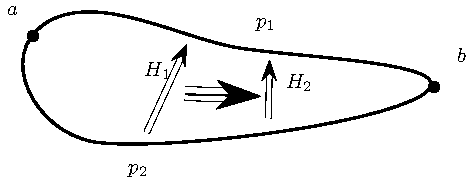
\includegraphics{path2}  
  \caption{Paths: $a$ and $b$ are points, $p_1$ and $p_2$ paths, $H_1$
  and $H_2$ homotopies.}
  \label{fig:paths}
\end{figure}
Indeed, that interpretation allows to explain all properties of
identity types.
\begin{itemize}
\item The equality $1_x$ is just the constant path 
  \[ \fonction{1_x}{[0,1]}{A}{t}{x} \]
\item The inverse $\inv \bullet$ is the function changing a path $f$ into
  \[ \fonction{g}{[0,1]}{A}{t}{f(1-t)} \]
\item The concatenation $\concat\bullet\bullet$ is the function
  changing paths $f$ and $g$ into
\[ \fonction{h}{[0,1]}{A}{t}%
  { \left\{
    \begin{array}{ll}
      f\left(2t\right) &\text{if } t\in[0,\nicefrac12] \\
      g\left(2t-1\right) &\text{if } t\in [\nicefrac12,1] 
    \end{array}
  \right.}
\]
\item A path between paths $f$ and $g$ between points $x$ and $y$ is a
  continuous function
  \[ 
    \fonction{H}{[0,1]²}{A}{(u,v)}{H(u,v)}
  \]
  such that $H(t,0) = f(t)$, $H(t,1) = g(t)$, $H(0,s)=x$ and
  $H(1,s)=y$. 
  A homotopy is then a continuous deformation of $f$ into $g$, fixing
  the ending points $x$ and $y$.
\end{itemize}

The table~\ref{fig:3pw} summarize the three points of view (type
theoretic, groupoidal, homotopy theoretic). In the rest of the thesis,
we will use any of the following name (\eg{} we will talk about
``points of a type'', ``path betwenn inhabitants'', \etc{}).

\begin{table}[h]
  \centering
  \begin{tabular}{|l|l|l|}
    \hline
    Type theory & Homotopy theory & $\omega$-groupoid \\
    \hline \hline
    Type & Topological space & $\omega$-groupoid \\
    \hline
    Inhabitant & Point & Object \\
    \hline
    Equality & Path & Morphism \\
    \hline
    $\idpath_x$ & Constant path & Identity morphism \\
    \hline
    $\inv\bullet$ & Inverse path & Inverse morphism \\
    \hline
    $\concat\bullet\bullet$ & Concatenation of paths & Composition of
                                                       morphisms \\
    \hline
    Equality between equalities & Homotopy & $2$-morphism\\
    \hline
  \end{tabular}
  \caption{Three points of view about HoTT}
  \label{fig:3pw}
\end{table}


What homotopy theorists love to do is to compute fundamental groups
(\ie{} the group of paths between two points) of
different spaces~(\cite{wangxu}\todo[fancyline]{These references
  were added without even opening them. Maybe a check would be good}
\cite{hutchings2011introduction}). We
can then categorized spaces with the level at which their homotopy
groups become trivial. Voevodsky has realized that this notion admits
a compact inductive definition internal to type theory, given by
\begin{defi}[Truncated types]
  $\IsType n$ is defined by induction on $n\geqslant -2$:
  \begin{itemize}
  \item $\IsType {(-2)}(X)$ if $X$ is a contractible type, \ie{} $X$
    is inhabited by $c:X$, and every other point in $X$ is connected to $c$.
  \item $\IsType {(n+1)}(X) \defeq \prod_{x,y:X} \IsType n (x=y).$
  \end{itemize}
  Then, $\Type_n \defeq \sum_{X:\Type} \IsType
  n(X)$\nomenclature{$\Type_n$}{Type of $n$-truncated types}.
\end{defi}

For the first values of $n$, there are different names:
$(-2)$-truncated types are called {\em contractible types},
$(-1)$-truncated types are called {\em h-propositions},
$0$-truncated types are called {\em h-sets}. Following this,
$\IsType{(-2)}$ is just $\Contr$, $\IsType{(-1)}$ is just $\IsHProp$
and $\Type_{-1}$ is $\HProp$, and $\IsType0$ is just $\IsHSet$ and
$\Type_0$ is $\HSet$. An explanation of this terminology might be
helpful. Contractible types are types, inhabited by a center $c$, with
paths between any point and $c$. A kind of magic thing about
contractible types is the lemma
\begin{lem}
  If $A:\Type$ is contractible, then for any $x,y:A$, the type $x=y$
  is contractible.
\end{lem}
Inductively, it means that paths types of any level over a contractible
type is contractible. It can be seen as the fact that a contractible
type contains only one point $c$, for which there is only one path
$c=c$, \etc{} The canonical example of contractible type is $\one$,
and actually, any contractible type is equivalent to $\one$.
Then, h-propositions are types where any two points are connected by a
path. The only difference with contractible types is that we allow the
type not to be inhabited. H-propositions are then proof-irrelevant
types, in the sense that under the propositions-as-types principle,
any points $x$ and $y$ in an $\HProp$ are equal, with a unique
equality, which is thus irrelevant.
\begin{lem}[Example of h-propositions]
  The following types are h-propositions:
  \begin{itemize}
  \item $\zero,\one$
  \item $\IsEquiv(f)$ for any $A,B:\Type$ and $f:A\to B$.
  \item $\IsType n(A)$ for any type $A:\Type$ and truncation index $n$.
  \end{itemize}
\end{lem}
Now, by definition, h-sets are types for which identity types are in
$\HProp$. The world of h-sets can thus be seen as the ``usual
mathematical'' world, as it satisfies proof-irrelevance.

The $n$-truncated types are stable under a lot of operations, as:
\begin{lem}
  Let $n\geqslant -2$ be a truncation index. Then
  \begin{itemize}
  \item If $A:\Type_n$ and $x,y:A$, then $\IsType n (x=y)$.
  \item If $A:\Type_n$ and $B:A\to\Type_n$, then $\IsType n
    \left(\sumD x A {B\, a}\right)$.
  \item If $A:\Type$ and $B:A\to\Type_n$, then $\IsType n \left(\prodD
      x A {B\, a}\right)$. Note that the source type needs not to be truncated.
  \item If $X:\Type_n$, $Y:\Type$ and $X\simeq Y$, then $\IsType
    n(Y)$.
  \item If $X:\Type_n$, then $\IsType{(n+1)}(X)$.
  \item We have $\IsType{(n+1)}{\Type_n}$.
  \end{itemize}
\end{lem}

\begin{rmq}
Some types are not $n$-truncated for any
$n$~\cite[Example 8.8.6]{hottbook} ; it is highly suspected for
example that the sphere $\mathbb S^2$ is one of
these $\infty$-truncated types (it is at least true in homotopy theory).  
\end{rmq}


This stratification of types induces a stratification of functions. A
function $f:A\to B$ is said to be $n$-truncated if all its homotopy
fibers $\fib f b$ are $n$-truncated. If $B:\Type$, a type $A$ together
with a $n$-truncated map $f:A\to B$ will be called a $n$-subobject of $B$.

As in~\cite{sets_in_hott}, we can define a sequence of subobject
classifiers, namely, $\Type_n$ classifies $n$-subobjects of a type
$B$, in the sens that there is an equivalence
\[\Xi : \sumD A \Type {\sumD f {A\to B} {\prodD b B
{\IsType n\
\fib{f}{b}}}} \xrightarrow{\sim} 
 (B \to \Type_n)\]
such that the diagram
\[
\xymatrix{
  A \ar[r]^{\hspace{-1em} t_f} \ar[d]_f & \Type_n^\bullet \ar[d]^{\pi_1}\\
  B \ar[r]_{\hspace{-1em} \chi_f} & \Type_n
}
\]
is a pullback for any $f$ with
 $n$-truncated homotopy fibers where $\Type_n^\bullet \defeq
 \sumD A \Type A$ is the universe of pointed
$n$-truncated types and 
\[ t_f = \lambda a,~(\fib{f}{f(a)},(a,\mathrm{idpath})). \]

We will use the equivalence $\Xi$ to define $n$-subobjects of a type
$B$ either as a $n$-truncated map $A\to B$, either as a characteristic
map $\chi:B\to\Type_n$.
\subsection{Truncations}
\label{ssec:trunc}

We present here a way to change any type into a $n$-truncated type, using
truncations. The interested reader can read Nicolai Kraus' PhD
thesis~\cite{phdkraus} consecrated to truncation levels in HoTT.

Let $n\geqslant -1$ be a truncation index. The $n$-truncation of a
type $A$ is the
higher inductive type $\|A\|_n$ \nomenclature{$\Vert\cdot\Vert$}{$n$-truncation of types}
 generated by
\[
  \left|
    \begin{array}{lll}
      \tr_n &:& A \to \|A\|_n \\
      \alpha_{\tr}^n &:& \IsType n (\|A\|_n)
    \end{array}
  \right.
\]
If $a:A$, $\tr_n(a)$ will be noted $|a|_n$.
The elimination principles are:
\begin{lem}[Elimination principle of truncations]\label{lem:trunc_elim}
  Let $A:\Type$ and $n\geqslant -1$ be a truncation index.
  \begin{itemize}
  \item If $P:\Type$ such that $\IsType n(P)$ and $f:A \to P$, then
    there is a map
    \[|f|_n : \|A\|_n \to P\]
    such that for all $a:A$, $|f|_n(|a|_n) \equiv f(a)$.
  \item If $P:\|A\|_n \to \Type$ such that $\prodD x {\|A\|_n}
    {\IsType n (P\, x)}$ and $f:\prodD a A {P(|a|_n)}$, then there is
    a dependent map
    \[|f|_n : \prodD x {\|A\|_n} {P\, x}\]
    such that for all $a:A$, $|f|_n(|a|_n) \equiv f(a)$.
  \end{itemize}
\end{lem}
\nomenclature{$\vert\cdot\vert_n$}{$n$-truncation of terms or arrows}
Basically, this induction principle says that $\|A\|_n$ has contains
as much data about $A$ than $A$ itself, but it can only be used to
define a $n$-truncated type. It can be expressed as the following
universal property:
\begin{lem}[Universal property of truncations]
  Let $A:\Type$ and $P:\Type_n$. Then the map
\todo[fancyline]{Check post or pre}
\[
  \fonction{\precompose_{\tr_n}}{A\to P}{\|A\|_n \to P}{f}{f \circ \tr_n}
\]
is an equivalence.
\end{lem}
We will see in chapter~\ref{chap:modalities} that all $(\IsType
n,\|\bullet\|_n)$ define {\em modalities}. In particular, every
truncation index $n$ yields a factorization system:

\begin{prop}
  Let $n\geqslant -1$ a truncation index. Then any map $f:A\to B$ can
  be factored as a $n$-connected map followed by a $n$-truncated map,
  where a map is $n$-connected if for all $b:B$, $\|\fib f b\|_n$ is contractible.
\end{prop}

In the rest of this thesis, we will only use this result with
$n=-1$. In that case, $(-1)$-truncated functions are called {\em
  embeddings}, and $(-1)$-connected functions are called {\em
  surjections}. The factorization of a map $f:A\to B$ is given by
\[
  \xymatrix{
    A \ar[rr]^f \ar[rd]^{\widetilde f} && B \\
    & \im(f)  \ar[ru]^{\pi_1} &
  }
\]
\begin{align*}
  \im(f) &\defeq \sumD b B {\left\| \sumD a A {f\, a = b}
  \right\|_{-1}} \\
  \widetilde f &\defeq \lambda a:A,\, \left(f\, a,\left|(a,1_b)\right|_{-1}\right)
\end{align*}

%%% Local Variables:
%%% mode: latex
%%% TeX-master: "main"
%%% End:
